%%%%%%%%% NEW SECTION: INTRODUCTION %%%%%%%%%

\section{Introduction}
The CRIMI \textbf{(Chris's ..... Interferometer)} is an infrared Fourier transform spectrometer, made by Chris de Jonge, under supervision of Dr. Andrey Baryshev. The spectrometer is designed to be used in a vacuum, as water molecules and other abundant molecules absorb large parts of the infrared spectrum.

%Doe hier ook een plaatje van een FTS (kun je van WIKIPEDIA halen). doel van je stage was:
%aansturing van linear stage
%grafische user interface
%data processing (FFT algorithmes + windowing)
%Zet in deze introductie ook een formule en plaatje met spectrum en interferogram.
%Verder is het goed om hier ook aan te geven hoe padlengte de resolutie bepaalt, en minimale stapgrootte de hoogste frequentie.

\subsection{Fourier Transform}

\begin{figure}
 \begin{center}
  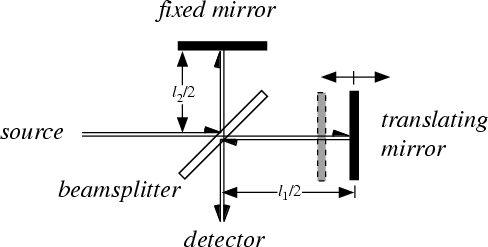
\includegraphics[width=0.8\textwidth]{figures/fts.png}
  \caption{A simple Fourier transform spectrometer (FTS). Path length differences are created by moving parts of the set-up.  From \cite{wolf}.}
  \label{fig:fts}
 \end{center}
\end{figure}

A Fourier transform spectrometer (FTS) works on the interference and Fourier principles. A moving beam-splitting mirror provides a difference in distance travelled by the two beams of light, which gives an interference pattern when recombined. The spectrometer setup measures the intensity of the combined signal as a function of position. A simple Fourier transform gets from this position data the intensity per wavenumber. The distance ($\delta$) and wavenumber ($\tilde{\nu}$) are together called a Fourier transform pair, because one is the inverse of the other:

\[
 \tilde{\nu} = \frac{1}{\delta},
\]

and from this the frequency $f$ can be computed: $\tilde{\nu}\cdot c=f$.

To measure this interference pattern, measurements at equally spaced distances are taken for a chosen measurement length. \textbf{[wat wil ik hier dan mee zeggen joh?]}

\begin{figure}
 \begin{center}
  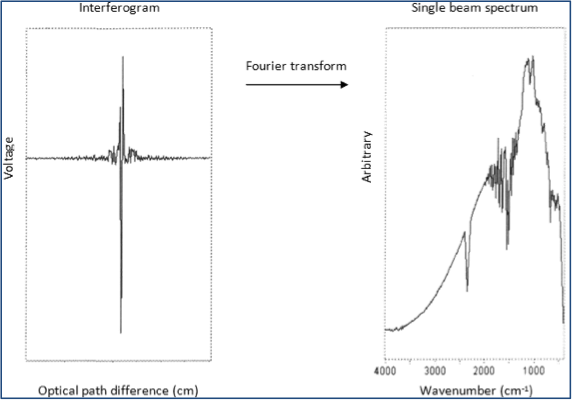
\includegraphics[width=0.8\textwidth]{figures/randomfouriertransform.png}
  \caption{The Fourier transform of an interferogram gives the spectrum. From \cite{ucdavis}.}
  \label{fig:fouriertransform}
 \end{center}
\end{figure}

The goal of this internship was to write software to guide the linear stage in making measurements, design a graphical user interface for easy user access and do some processing on the acquired data: fast Fourier transforms and windowing. As a result, I have written a program in Python that automatically takes a complete measurement with this spectrometer. The program has scan length and stepsize, or equivalent resolution and maximum frequency, for input, and outputs the raw data in csv format.

The spectrometer needs a few devices to function: a controller to move the stage, a lock in amplifier, and a device to actually measure the power of the radiation. This report will not deal with the actual measuring device, as the setup is independent of that. %It suffices to say that the test measurements were done with a helium-cooled bolometer (and not in a vacuum environment).

\begin{itemize}
\item Algemene inleiding over de CRIMI. (sortof done)
\item Iets met dat het programma voor windows geschreven is (serial ports zijn com-ports).
%z\item dingen over waarom een fts gebruiken (fourier $\rightarrow$ dus informatie over meerdere frequenties in 1x).
%\item \textbf{check measurement 20121005-1725!}
\item something about the lock in technique?
\end{itemize}

\subsection{Hardware}

As already mentioned, the spectrometer setup makes use of a few different devices. The controller to move the stage in is the PI C867.160 controller. The lock in amplifier in use is the SR510. A third device is needed to be able to communicate with the lock in amplifier from any computer: a GPIB-Ethernet adapter. This device counteracts the need for a special GPIB circuit card in the computer. Figure~\ref{fig:hardware} shows the different devices. All three are hardcoded into the software. This means unfortunately that the software does not automatically work with e.g. the SR530 lock in amplifier, or with a direct GPIB connection to the computer.

%\begin{itemize}
%\item Noem de PI Controller voor de stage, de EthernetAdapter (hoe heet dat ding) en de lock in, SR510.
%\item Zeg iets over switch 6 van de lock in amplifier.
%\end{itemize}

\begin{figure}[h!tb]
	\begin{center}
		\subfloat[The controller for the stage from PI.]{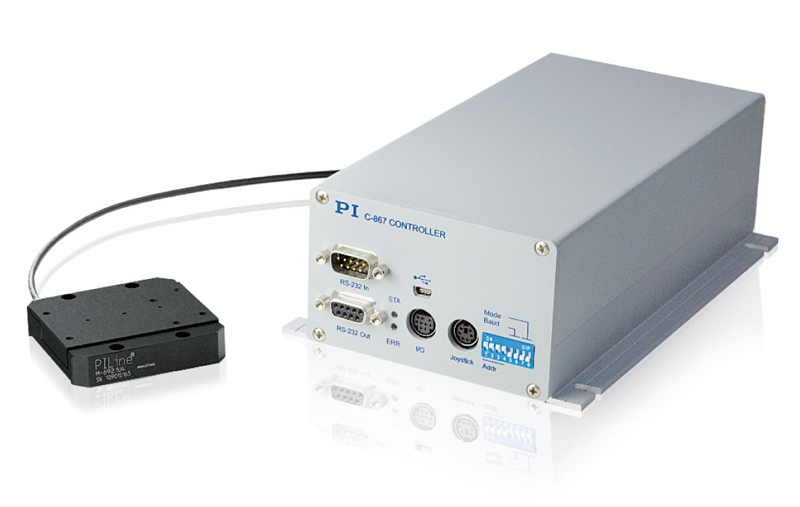
\includegraphics[width = 0.45\textwidth]{figures/pi_c867_160.jpg}}
		\qquad
		\subfloat[The SR510 lock in amplifier.]{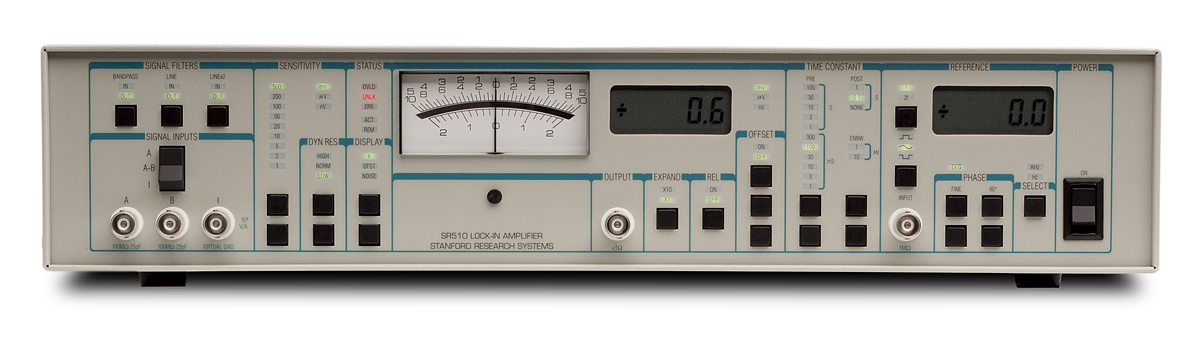
\includegraphics[width = 0.45\textwidth]{figures/SR510_FPlg.jpg}}
		\qquad
		\subfloat[The GPIB-Ethernet Controller.]{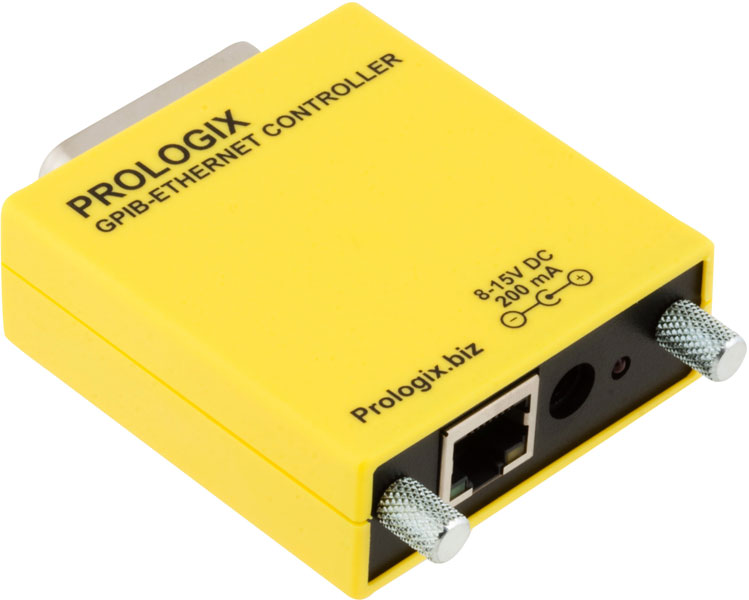
\includegraphics[width = 0.4\textwidth]{figures/GPIB-Ethernet-back.jpg}}
		\caption{The hardware. Pictures from \cite{PI}, \cite{SR}, and \cite{prologix}.}
		\label{fig:hardware}
	\end{center}
\end{figure}

It is important to mention that on the SR510 the DIP-switches need to be in a different configuration than the `example' configuration as mentioned in its manual on page 7. For fast readout, SW1 switch 6 should be in the `up' position instead of in the `down' position, to suppress echoing over the, in this setup unconnected, RS232 connection. The SW2 switches are not of importance in this setup, as no RS232 connection is used. See figure~\ref{fig:SR510_back} for the location of this switch.

\begin{figure}
 \begin{center}
  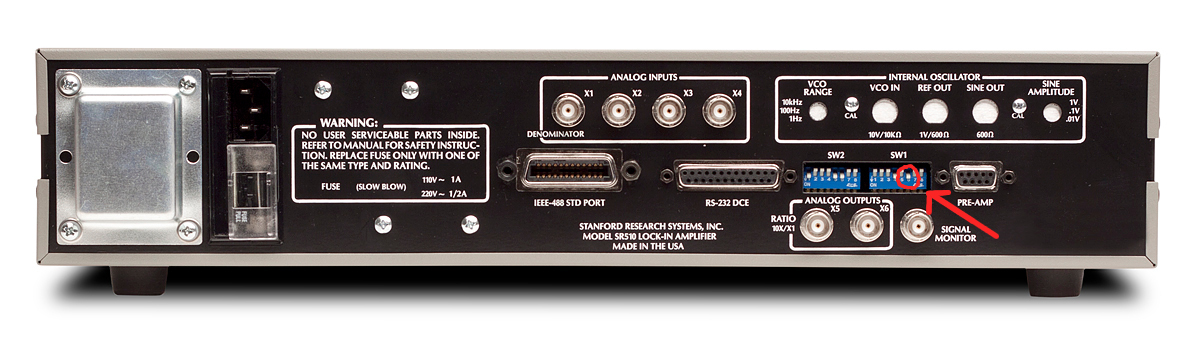
\includegraphics[width=\textwidth]{figures/SR510_Rear_circle.jpg}
  \caption{The back plate of the SR510 lock in amplifier. Encircled is SW1 switch 6. For fast performance, this switch should be in the `up' position. Picture from \cite{SR}.}
  \label{fig:SR510_back}
 \end{center}
\end{figure}


%Plaatje voor GPIB-Ethernet Controller van http://prologix.biz/images/detailed/0/GPIB-Ethernet-back.jpg
%Plaatje voor PI Controller: http://www.physikinstrumente.com/en/primages/pi_c867_160_m692_i4c_o.jpg
%Plaatje Lock In Amplifier: http://www.thinksrs.com/assets/instr/SR510530/SR510_FPlg.jpg

\subsection{Python}
Python is an interpreted, interactive, object-oriented programming language \cite{python}. It is open source and free, and easy to learn. Python runs on Windows, Linux/Unix and Mac OS X. It has an active community that contributes a large number of libraries for various tasks, e.g. numerical mathematics and hardware interfacing.

Python has the distinct advantage over programming languages such as LabVIEW that it is backwards compatible. Old code written in previous versions is in many cases still executable in newer Python versions, and as the files are plain text, it will be always readable in any editor. So even when old code cannot be executed anymore, it can still be modified to comply with newer standards.

This software is written in Python version 2.7. The extra (non-native) packages needed for the program are \verb!PySerial! to open a serial port for the PI-controller and \verb!wxPython! to make the GUI. For this last task \verb!wxFormbuilder!, an open source GUI designer which emits Python code, was also used. The other imported packages are part of the core Python distribution.
